% Created 2017-03-11 Sat 18:34
\documentclass[12pt]{amsart}
                        \usepackage[all]{pabmacros}
\usepackage[utf8]{inputenc}
\usepackage[T1]{fontenc}
\usepackage{fixltx2e}
\usepackage{graphicx}
\usepackage{longtable}
\usepackage{float}
\usepackage{wrapfig}
\usepackage[normalem]{ulem}
\usepackage{textcomp}
\usepackage{marvosym}
\usepackage[nointegrals]{wasysym}
\usepackage{latexsym}
\usepackage{amssymb}
\usepackage{amstext}
\usepackage{hyperref}
\tolerance=1000
\usepackage{amsmath}
\usepackage[bibstyle=alphabetic,citestyle=alphabetic,backend=bibtex]{biblatex}
\makeatletter
\def\blx@maxline{77}
\makeatother
\bibliography{refs}
\AtEveryBibitem{\clearfield{doi}}
\AtEveryBibitem{\clearfield{url}}
\AtEveryBibitem{\clearfield{issn}}
\renewcommand*{\bibfont}{\footnotesize}
\renewcommand\maketitle{}
\usepackage{enumitem}
\usepackage{setspace}
\usepackage[margin = 6mm]{geometry}
\pagenumbering{gobble}
\pagestyle{empty}
\renewcommand*{\bibfont}{\footnotesize}
\date{}
\title{D1 Project Description}
\hypersetup{
  pdfkeywords={},
  pdfsubject={},
  pdfcreator={Emacs 24.5.1 (Org mode 8.2.10)}}
\begin{document}

\maketitle


\smallskip\noindent{\Large\textbf{\textsc{Project Title}}}
\label{sec-1}
Analysis and geometric techniques for fully non-linear problems in geometry and PDE.

\smallskip\noindent{\Large\textbf{\textsc{Aims And Background}}}
\label{sec-2}
Geometric evolution equations are ubiquitous and have been used to extraordinary effect in solving many important problems in geometry and topology.  Perhaps the most famous, is the resolution of the \poincare{} conjecture by Hamilton and Perelman \cite{MR2334563}.  Other, equally striking (mathematically, perhaps if not sensationally) results are the $1/4$ pinched sphere theorems (see \cite{MR2738904} for a recent survey article or \cite{MR2760593} for a more comprehensive account), Cao's proof of the Calabi conjecture \cite{MR799272} and two different proofs of the Riemannian Penrose inequality \cite{MR1916951, MR1908823}.  Geometric flow type techniques were also recently used to prove the fundamental gap conjecture \cite{MR2784332} whilst  the Ricci flow on surfaces can also be used to prove the uniformisation theorem \cite{MR2729306}.

Such results depend crucially on careful analysis of asymptotics and singularity formation. Innovative isoperimetric comparison techniques were introduced in \cite{MR2729306,MR2794630,MR2843240,pbthesis,Bryan} Prof. Ben Andrews and I to obtaining very direct proofs that arbitrary initial configurations converge smoothly to the model, constant curvature configuration. These results then yield proofs of the famous uniformisation theorem classifying all closed surfaces by genus, and also the classical isoperimetric inequality stating that among all planar figures of a given area, the circle has the least perimeter.

In three dimensions, the \poincare{} conjecture mentioned above fits into a larger scheme known as the Thurston Geometrisation Conjecture and this is in fact what Hamilton and Perelman proved. Roughly speaking, this conjecture says any compact three dimensional manifold may be decomposed into smaller simpler pieces, and that each of these pieces is one of eight possible types - the so called \emph{Prime manifolds}. The manifolds include in particular the standard Euclidean, Spherical and Hyperbolic geometries. Such a decomposition allows one to study these pieces separately and is a great boon given the otherwise complex topology of three-manifolds. In particular, the negatively curved manifolds form the largest class of prime manifolds and deeper questions on these objects are not well suited to Hamilton's and Perelman's approach based on the Ricci flow which is most effective in positive curvature. To remedy the situation Hamilton and Chow introduced the Cross Curvature Flow \cite{MR2055396}, a fully non-linear equation that preserves the property of negative curvature. Only scattered results are known for this flow so far, but all support the conjecture that any negatively curved manifold will smooth converge to a constant curvature, \emph{hyperbolic manifold}. Such a result would imply, for example, that the space of negative curvature metrics on a hyperbolic manifold is path connected and hence any such manifold may be seen as a perturbation of the constant curvature hyperbolic manifold thus revealing hidden simplicity in the topology of these mysterious negatively curved spaces.

Another approach to these types of problems is to study ancient solutions, solitons and the closely related Harnack inequality. It has been known for some time that ancient solutions, and solitons in particular model singularity formation and hence studying such special solutions lends tremendous insight into the sort of problems described above. Dr. Mohammad Ivaki, Dr. Julian Scheuer and I have developed considerable apparatus \cite{BIS4,2016arXiv160401694B,2015arXiv150802821B,2015arXiv151203374B} for studying ancient solutions and obtaining Harnack inequalities in Riemannian backgrounds, a very surprising and difficult result given the non-linearity introduced by the curvature of the background space, and the only major new result on such inequalities this century. Moreover, very strong classification results for ancient solutions were obtained via geometric methods showing for example that for any heat-type geometric flow on the sphere, the only ancient, convex solutions are spherical caps, suggesting that in positive curvature, the space of such solutions is very rigid. By linear stability analysis, one may approximate a minimal surface by an ancient solution of the Mean Curvature Flow and the classification results may then be applied to obtain area bounds for minimal surfaces in terms of topological properties such as the Morse index which measures the number of independent directions in which a minimal surface may be deformed to strictly decrease area.

The \textbf{aim} of this proposal is to extend the innovative and powerful methods described above to a broad variety of actively studied problems with applications to hyperbolic manifold topology, isoperimetric inequalities, and minimal surfaces.

\begin{enumerate}[label=\textbf{(\Alph*)}]
\item Examine the connections between geometric evolution equations and isoperimetric comparisons, obtaining comparisons and quantifying asymptotic singulariy formation for a variety of geometric evolutione equations (joint with Prof. Ben Andrews and Prof Mariel \saez{}).
\item Develop a theory of the Cross Curvature Flow and apply it to obtain a topological classification of hyperbolic manifolds (joint with Dr. Mohammad Ivaki and Dr. Julian Scheuer).
\item Perform stability analysis of ancient solutions to curvature flows and classify such solutions. In particular, apply these results to obtain conjectured area bounds for minimal surfaces and explore the connections between curvature flows and the conformal geometry of the sphere (joint with Dr. Mohammad Ivaki and Dr. Julian Scheuer).
\end{enumerate}

\noindent More details aims and background for each project follow.

\noindent\textbf{Project A: Isoperimetric Comparisons}
\label{sec-2-1}
The classic isoperimetric inequality states that the figure in the plane with least perimeter bounding a given area is a circle. This result has been known since antiquity by the name Dido's problem who was tasked with enclosing the greatest amount of area given a fixed perimeter. In the 20th century, isoperimetric inequalities comparing the perimeter of a figure with it's enclosed area were obtained for constant curvature spaces. The situation is illustrated in figure \ref{fg:const_curve_isoperimetric}. The latter part of the 20th century and early parts of this century saw the beginning of results for spaces with variable curvature \cite{MR1699261,MR1661278,MR1883725,MR1417620}.

\begin{figure}[htb]
\centering
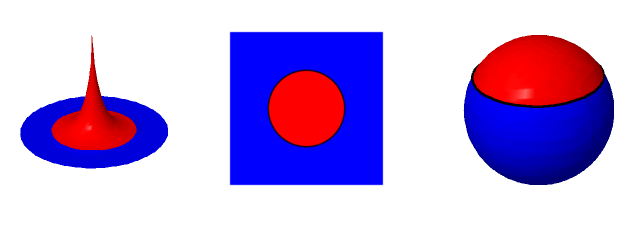
\includegraphics[width=0.7\textwidth]{img/const_curve.png}
\caption{\label{fg:const_curve_isoperimetric}From left to right: an isoperimetric region (red) in a constant negative curvature surface, the plane, and the sphere.}
\end{figure}

The isoperimetric profile of a Riemannian manifold was introduced in the 1980's \cite{MR875084,MR999971} to study isoperimetric inequalities on Riemannian manifolds. It is a function that gives the least perimeter bounding a given area $x$, and is defined by
\[
I(x) = \inf\{\operatorname{Area} (\bdry{\Omega}) : \operatorname{Vol}(\Omega) = x\}.
\]
Thee sharpest possible isoperimetric inequality on a Riemannian manifold comparing the $n-1$ dimensional area of a figure with it's enclosed $n$ dimensional volume is recorded in $I$:
\[
\operatorname{Area}_{n-1} (\bdry{\Omega}) \geq I(\operatorname{Vol}_n(\Omega))
\]
For example the classic isoperimetric inequality implies that the isoperimetric profile of the plane is $I_{\RR^2}(x) = \sqrt{4\pi x}$, of the $2$-sphere is $I_{\sphere^2}(x) = \sqrt{4\pi x - x^2}$ and of the hyperbolic plane is $I_{\HH^2} (x) = \sqrt{4\pi x + x^2}$. We have the obvious inequalities,
\[
I_{\sphere^2} < I_{\RR^2} < I_{\HH^2}
\]
which exhibits the general expected phenomena that increasing curvature allows one to enclose more area for a given perimeter which is also evident in figure \ref{fg:const_curve_isoperimetric}. A variant of Dido's problem says that she encircled a hill (positive curvature) to obtain more area compared with a flat plane (zero curvature) suggesting that she was qualitatively aware of the connection to curvature.

A major outstanding conjecture in this area is the Aubin-Cartan-Hadamard conjecture \cite{MR0448404, MR936419} bounding the isoperimetric profile of a negatively curved manifold by the constant curvature model space profile. Classically, this has been proven in dimension 2 \cite{zbMATH02588223}, dimension 3 \cite{MR1156385,MR2167269} and dimension 4 \cite{MR608287} (for $K_0 = 0$ only), but still remains outstanding in general.

For a curve in the plane, similar to the isoperimetric profile, we may define the \emph{chord-arc profile} as the least distance between any points on the curve of a given arc-length along the curve):
\[
Z(x) = \inf\{d(p, q) : \ell(p, q) = x\}
\]
where $d$ denotes the distance between two points in the plane and $\ell$ denotes the distance along the curve.

Once more, curvature plays a role in this profile as depicted in figure \ref{fg:chord_arc} with larger curvature forcing greater length along the curve as compared with an arc of fixed distance between two points on the curve.

\begin{figure}[htb]
\centering
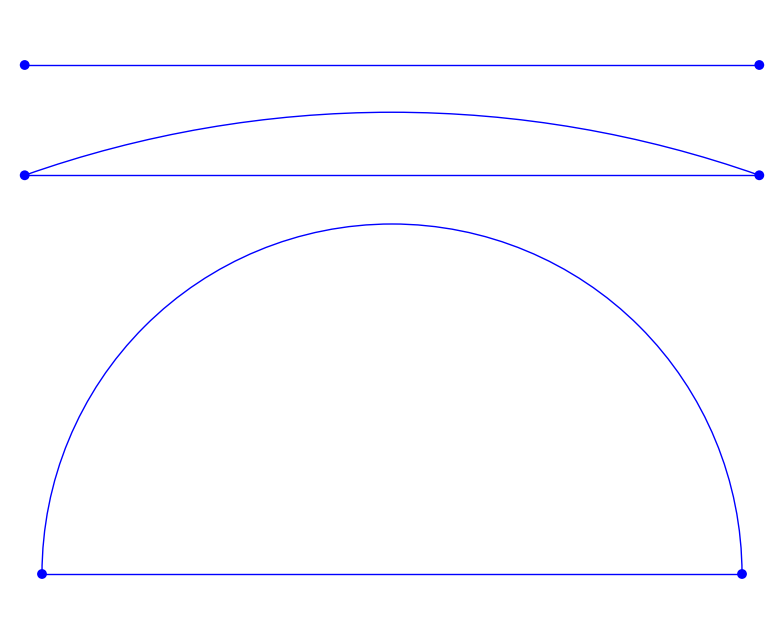
\includegraphics[width=0.5\textwidth]{img/chord_arc.png}
\caption{\label{fg:chord_arc}From top to bottom, a straight line has equal distance and arc-length, small curvature implies slightly larger arc-length, and large curvature has much larger arc-length.}
\end{figure}

The (planar) Curve Shortening Flow is the evolution equation,
\[
\partial_t \gamma = - \kappa\nu
\]
for a smooth, one-parameter family of immersed curves $\gamma_t \subset \RR^2$ in the plane with $\kappa$ is the geodesic curvature with respect to a smooth choice of unit normal, $\nu$. The most famous result regarding this equation is that closed, embedded curves collapse to a point in finite time, smoothly converging to a circle after rescaling to keep the total length fixed \cite{MR840401,MR906392}. In \cite{MR2794630}, with Prof. Ben Andrews and using the chord-arc profile, I proved a distance comparison principle leading to a curvature bound and subsequent direct proof of this result. A related flow is the flow,
\[
\partial_t \gamma = -\kappa\abs{\kappa}^{\alpha-1} \nu.
\]
This flow has greater non-linearity than the Curve Shortening Flow, and owing to the absolute value, has non-smooth speed for non-convex curves at points where the curvature vanishes. Convergence results for convex curves (where the speed is smooth) have been obtained \cite{MR1660843}, but the general case remains open and may be approached using distance comparison methods Prof. Ben Andrews and I developed.

The distance comparison argument in \cite{MR2794630} applies also to the Curve Shortening Flow of networks, a topic that has received considerable attention in recent years \cite{MR2394409,MR2075985,MR2763716}. In this context, a network is an embedded graph in the plane. Each edge has vertices either lying on the boundary of a convex body (or on the circle at infinity), or meets precisely two other edges at a vertex and with equal angles of $2\pi/3$ (\emph{triple condition}). See figure \ref{fg:network}.
\begin{figure}[htb]
\centering
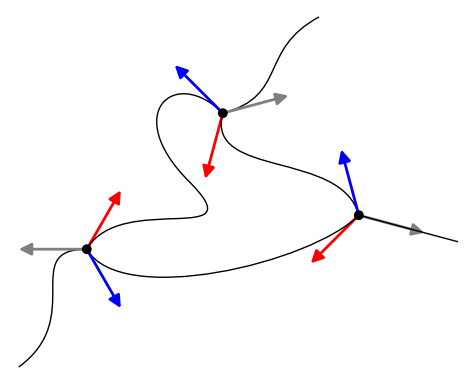
\includegraphics[width=0.4\textwidth]{img/network.png}
\caption{\label{fg:network}A network with three nodes satisfying the triple condition.}
\end{figure}

The flow is by curve shortening on the interior of the edges, subject to the boundary triple condition. Such a flow was initially studied to model annealing metals \cite{MR0078836} and is of interest in materials science. The flow, like in the smooth case, is also the gradient flow of the length functional, from which perspective the triple condition arises naturally. This part of the project aims to prove that singularity formation can only occur when an edge has length collapsing to zero, confirming the so-called multiplicity one conjecture.

This project's \textbf{aims} are:
\begin{enumerate}[label=\textbf{(A.\arabic*)}]
\item Investigate isoperimetric comparisons in negatively curved manifolds.
\item Define Homogeneous Curve Shortening Flow for non-convex curves and obtain convergence results by distance comparison.
\item Develop distance comparison for the Curve Shortening Flow of networks and investigate singularity formation.
\end{enumerate}

\noindent\textbf{Project B: Cross Curvature Flow (XCF) And Hyperbolic Manifolds}
\label{sec-2-2}
Let $E = \operatorname{Ric} - \tfrac{1}{2} \operatorname{R} g$ denote the Einstein tensor of a Riemannian manifold $(M, g)$. We define the endomorphism $\mathcal{E}$ of the tangent bundle $TM$ by $E(X, Y) = g(\mathcal{E}(X), Y)$, and Einstein-Ricci tensor,
\[
\operatorname{Ric}_E (X, Y) = \operatorname{Tr} \left[Z \mapsto \operatorname{Rm} (\mathcal{E}(Z), X) Y\right],
\]
Then the XCF is the evolution equation,
\[
\partial_t g = -2 \operatorname{Ric}_E.
\]
This is a parabolic equation and preserves negative sectional curvature \cite{MR2055396,MR2207496}. In three dimensions, negative sectional curvature corresponds to $E$ being a metric (positive definite bi-linear form), and the Einstein-Ricci tensor is nothing more than contracting the Riemann tensor, not with the metric $g$, but with the metric $E$. Note that contracting with $g$ gives the usual Ricci tensor and the flow becomes the celebrated Ricci flow. The XCF may in fact be defined in other equivalent ways that agree in three dimensions, but not in higher dimensions in a similar manner to the agreement of the Ricci flow and Yamabe flow in two dimensions. These higher dimensional flows have yet to be studied, opening the door for significant results in hyperbolic geometry of higher dimensions.

As noted in \cite{MR2602839}, hyperbolic manifolds are the largest class of prime manifolds, but it's not yet known whether this space is contractible, or even connected. The Cross Curvature Flow (XCF) was introduced in \cite{MR2055396} in the hopes of deforming negatively curved metrics $g_0$ on a compact three-manifold $M$ to constant curvature metrics. Such a conjectured result would confirm contractibility of the space of negatively curved metrics on a hyperbolic manifold. Partial results for homogeneous manifolds and solid tori have been established \cite{MR2407107,MR2653711,MR2602839} as well as asymptotic stability near hyperbolic metrics \cite{MR2448593} in support of the conjecture.

This project's \textbf{aims} are:
\begin{enumerate}[label=\textbf{(B.\arabic*)}]
\item Prove the XCF deforms classes of strictly negatively curved metrics to constant curvature metrics.
\item Determine isoperimetric comparisons for the XCF.
\item Generalise the XCF to higher dimensions.
\end{enumerate}

\noindent\textbf{Project C: Ancient Solutions}
\label{sec-2-3}
It has long been understood that curvature flows and minimal surfaces are closely related, yet explicit applications to minimal surfaces have been minimal. In \cite{2016arXiv160401694B}, Dr. Mohammad Ivaki, Dr. Julian Scheuer and I proved the very general result that any convex, ancient hypersurface solution of a parabolic, geometric flow in the sphere must be a family of shrinking spherical caps emanating from an equator (a minimal surface) at $t=-\infty$ and collapsing to the north pole at $t=0$. To obtain similar results in a general Riemannian background, given an unstable minimal surface $M_0$, linear stability analysis implies that the space of ancient solutions converging backwards to $M_0$ as $t\to-\infty$ is a finite dimensional linear sub-manifold corresponding to the unstable eigenspace. Further analysis should show that there is unique mean convex ancient solution corresponding to the first eigenvalue which is simple (the eigenspace is one-dimensional).

Regularity theory of mean convex mean curvature flow has undergone significant development recently \cite{2013arXiv1304.0926H,MR3570481} allowing the geometric inequalities of \cite{MR1650335} to be applied to the unique mean convex mean curvature flow (which may undergo singularities previously hampering progress with this method) to obtain area control for $M_0$ in terms of the value of the first eigenvalue.

As a striking example of possible applications, we see that there is a five-dimensional family of ancient solutions emanating from a Clifford Torus in $\sphere^3$. The motion of this family is, to first order, by the canonical family of conformal transformations used in the resolution of the Willmore conjecture \cite{MR3152944}. This suggests a hitherto unknown connection between the conformal geometry of the sphere and the Mean Curvature flow with applications to Willmore surfaces.

This project's \textbf{aims} are:
\begin{enumerate}[label=\textbf{(C.\arabic*)}]
\item Classify ancient solutions of curvature flows in Riemannian backgrounds.
\item Prove area estimates for unstable minimal surfaces in terms of the space of unstable directions.
\end{enumerate}

\smallskip\noindent{\Large\textbf{\textsc{Project Quality And Innovation}}}
\label{sec-3}

\begin{itemize}
\item Brief summary of innovations.
\end{itemize}

\noindent\textbf{Isoperimetric Comparisons}
\label{sec-3-1}
\subsubsection*{Comparison theorems for the isoperimetric profile.}
\label{sec-3-1-1}



In \cite{Bryan,pbthesis,MR2843240,MR2794630}, a (parabolic) viscosity differential inequality for the isoperimetric profile is used to obtain a comparison principle for the isoperimetric profile evolving under curvature flows. The spatial version of this inequality is also used to investigate properties of the isoperimetric profile such as in positive curvature, concavity of the isoperimetric profile implies isoperimetric regions have connected boundary (see also \cite{MR1674097}). The Levy-Gromov isoperimetric inequality can also be proved using this approach \cite{MR3544942} and has been recently extended to RCD spaces \cite{MR3608721}, those metric measure spaces with lower Ricci bounds.

\noindent\textbf{The Cross Curvature Flow and hyperbolic manifolds (joint with Dr. Mohammad Ivaki and Dr. Julian Scheuer)}
\label{sec-3-2}
As noted in \cite{MR2602839}, hyperbolic manifolds are the largest class of prime manifolds. It's not known whether this space is contractible, or even connected. The Cross Curvature Flow (XCF) was introduced in \cite{MR2055396} in the hopes of deforming negatively curved metrics $g_0$ on a compact three-manifold $M$ to constant curvature metrics. Such a result would confirm contractibility of the space of negatively curved metrics on a hyperbolic manifold. Very little apart from short-time existence and uniqueness \cite{MR2207496} and partial results (e.g. \cite{MR2448593,MR2407107}) is known about solutions of the cross-curvature flow, but such results support the conjectured contractibility which is the aim of this section.

\noindent\textbf{Singularities, symmetries and ancient solutions of fully non-linear geometric evolution equations (joint with Dr. Mohammad Ivaki and Dr. Julian Scheuer)}
\label{sec-3-3}


\noindent\textbf{Isoperimetric Comparisons}
\label{sec-3-4}

An innovation of this project is the use of Isoperimetric comparisons which may then be used to tackle problems such as the Aubin-Cartan-Hadamard conjecture mentioned above. One possible approach is to deform regions by curvature flows such as the Mean Curvature Flow or the Inverse Mean Curvature Flow. This approach was taken in \cite{MR2420018} by using the mean-convex Mean Curvature Flow to prove the Euclidean isoperimetric inequality but suffered from the lack of suitable tools to analyse non-smooth flows. Such tools have been developed recently for example in \cite{MR3570481,2013arXiv1304.0926H} where regularity results and structure theorems have been more fully developed. In the radial model setting, isoperimetric inequalities have been proven using curvature flows \cite{MR3439091,2016arXiv160908238G}, whilst my collaborator has proven long-time existence results for inverse curvature flows in non-positively curved backgrounds \cite{MR3581327}. Combining these techniques and comparing singularity formation with the radial model in a similar manner to \cite{MR1650335} may be used to obtain suitable comparison results resolving the conjecture.

\noindent\textbf{Homogeneous Curve Shortening Flow}
\label{sec-3-5}

For the homogeneous Curve Shortening Flow, an innovation is to define approximating flows,
\[
\partial_t \gamma = -\kappa\abs{\kappa^2 + \epsilon^2}^{\tfrac{\alpha-1}{2}} \nu
\]
which are smooth, strictly parabolic flows. The next step is to obtain a priori estimates via two approaches: one for $\alpha \in (1/3, 1]$ and one for $\alpha \geq 1$. Both methods are applicable to the critical case of the Curve Shortening Flow, $\alpha = 1$, the first method being the distance comparison principle in \cite{MR2794630}.

For such flows, the comparison applies for \emph{operator monotone} functions which satisfy $A \geq 0 \Rightarrow f(A) \leq 0$ for matrix $A$, which restricts to $\alpha \leq 1$. The following differential inequality for the chord-arc profile holds in this case:
\[
\partial_t Z \geq 2 \frac{2^{\alpha+1}}{\left(\sqrt{1 - (Z')^2}\right)^{\alpha-1}} f(Z'') - \avg{f(\kappa) \kappa} \left(Z - Z'\ell\right) - Z' \int_{p_0}^{q_0} f(\kappa)\kappa ds
\]
where $f(y) = y\abs{y}^{\alpha-1}$ is the speed of the flow, $\avg{\cdot}$ denotes the mean value over the curve $\gamma$ and $(p_0, q_0)$ are points of given intrinsic length $\ell(p_0, q_0)$ achieving the infimum of extrinsic distance $d(p_0, q_0)$. Given the critical exponent $\alpha=1/3$ discussed above, it's expected that the curvature estimates obtained using the methods in \cite{MR2794630} should hold for $\alpha \in (1/3, 1]$. Supporting evidence for this conjecture is that the differential inequality is linearly stable around the round circle.

For the case $\alpha \geq 1$, the Harnack inequality may be used (similar to \cite{MR1094458}) to show that the approximating flows become convex in finite time whence the existing results for convex curves apply.

\noindent\textbf{Network Curve Shortening Flow}
\label{sec-3-6}

Prof. Mariel \saez I have shown that the comparison principle for the chord-arc profile developed in \cite{MR2794630} holds for networks after suitable modification to deal with the triple points. To preserve the coincidence of the vertices of the edges, a tangential component of velocity must be introduced, and geometric invariant of the flow implies only the value at the vertices is important. Let us write $\Delta v_m$ for the difference between this value at joining edges. Then the viscosity equation for the chord-arc profile is
\[
\partial_t Z \geq 4Z''+\bar{Q}(Z-xZ')+f'(\Delta Q(p,q)).
\]
where $\bar{Q}=\frac{1}{L}\int k^2 ds-\sum_{m=1}^n \Delta v_m$ and $\Delta Q(p,q)=\frac{1}{L}\int_p^q k^2 ds-\sum_{m=i_p}^{i_q} \Delta v_m$. The only difference with the smooth case is the introduction of the $\Delta v_m$ terms.

The aim here is to use construct suitable comparison functions in order to obtain a curvature bound similar to \cite{MR2794630}. The network flow has a number of differences to the smooth flow requiring further analysis. Two important differences are asymptotics of the chord arc profile differ from the smooth case while the triple points introduce new terms into the viscosity equation. However, though not explicitly articulated in \cite{MR2794630}, there is a powerful procedure for finding suitable comparison functions: make a similarity substitution using the profile of the self-similar solution in the viscosity equation. In the smooth case, this is the circle but in the network case there are multiple self-similar solutions and the comparison must take this into account. On the other hand, the correct asymptotics and additional terms arising from the triple points are automatically dealt with. The aim then is to complete this program and prove the major current outstanding conjecture, that the only singularities possible are of multiplicity one which follows readily from the chord-arc comparison.

\noindent\textbf{Cross Curvature Flow}
\label{sec-3-7}

The project on the Cross Curvature Flow and hyperbolic manifolds is highly innovative, identifying previously unknown deep structure and describing powerful techniques for understanding the geometry of hyperbolic manifolds similar to the Ricci flow's role in positively curve geometry. The extensions to higher dimensions and underlying algebraic structure have not previously been observed and will open up an entirely new approach to high dimensional hyperbolic geometry. Furthermore, the isoperimetric comparisons will demonstrate that the tremendous power of these methods has very broad applicability building upon my previous innovations.

\subsubsection*{Estimates}
\label{sec-3-7-1}


The conjectured asymptotic behavior of the XCF has been recently confirmed whenever $M$ locally isometrically embeds as a hypersurface into Minkowski space $\RR^{3,1}$ \cite{MR3344442}. The main observation there is that in such a situation, the embedded hypersurface evolves by the Gauss curvature flow. The obstruction to applying this method is the local, isometric embedding problem which is equivalent to isometrically embedding the universal cover of $M$ into $\RR^{3,1}$ which is not generally true.

In the locally isometrically embedible situation, with Doctor's Mohammad Ivaki and Julian Scheuer we obtained the Harnack inequality \cite{BIS4},
\[
\partial_t \sqrt{{\det} \mathcal{E}} - \frac{1}{\sqrt{{\det}\mathcal{E}}} \abs{\nabla \sqrt{{\det}\mathcal{E}}}_E^2  + \frac{3}{4 t} \sqrt{{\det}\mathcal{E}} \geq 0
\]
where $\abs{\cdot}_E$ refers to the norm with respect to the Einstein tensor $E$. An immediate application of this inequality is that negative sectional curvature is preserved by the flow since that corresponds to preserving $\mathcal{E}$ non-singular and the Harnack inequality implies that if $\mathcal{E}$ becomes singular, then $\nabla \mathcal{E}$ blows up. Moreover, combined with $C^0$ estimates, the Harnack inequality gives an alternate proof of the conjecture. In fact, all that is required is a Harnack inequality and not the isometrically embedible assumption. Proving the Harnack involves great computational complexity in the general case, though early computations show it is possible to obtain a Harnack under the assumption, $\nabla V$ is totally symmetric where $V (X, Y) = g(\mathcal{E}^{-1}(X), Y)$. In the locally embedible case this condition follows from the Codazzi equation, but does not necessarily imply local embedibility. These initial results are thus already more general than those in \cite{MR3344442} and will be an early output of the project.

\subsubsection*{Comparisons for the Einstein volume under the Cross Curvature Flow.}
\label{sec-3-7-2}



The aim is to derive a viscosity equation for the Einstein Isoperimetric Profile, giving the least area for a given volume as measured by the induced volume form and surface measure by the Einstein tensor:
\[
I_E (x) = \inf\{\operatorname{Area}_E (\Omega) : \operatorname{Vol}_E (E) = x\}.
\]
In \cite{MR2055396} it was shown that the Einstien volume is monotone along the flow, which suggests that as with the isoperimetric profile for the Ricci flow, this approach will prove quite powerful.

In the critical dimension three, one hopes to be able to exploit such topological invariants arising from the conformal-like structure of the cross curvature flow, as well as Hodge duality identifying vectors and two-vectors. The relevance here is that the Gauss-Bonnet theorem played a pivotal role in the proof of the isoperimetric comparison theorems for the Ricci flow in \cite{Bryan,MR2729306}. There, the theorem was applied to the second variation of perimeter of isoperimetric domains to obtain a viscosity equation for the isoperimetric profile which formed the basis of the comparison theorem. In three dimensions, a consequence of the Poincare-Hopf index lemma is that one always has a non-vanishing vector field $X$ at one's disposal, and by Hodge duality, also a non-vanishing two-vector field $\eta$ but a lack of exactness as measured by $H^1(M) \simeq H^2(M)$ is an obstruction and the aim is to quantify this topologically, similar to the way the Euler characteristic appears in the Gauss-Bonnet theorem.

\subsubsection*{Higher Dimensions}
\label{sec-3-7-3}

The definition given above for the XCF makes sense in any dimension. Moreover, there is another way to interpret the XCF. First recall above that the XCF is the equation,
\[
\partial_t g = -2 \operatorname{Ric}_E.
\]
Let us call this equation the \emph{Einstein Ricci Flow}. Now, let $\operatorname{adj} \mathcal{E}$ denote the adjugate of $\mathcal{E}$ defined as the $\wedge$ adjoint of $\wedge^{n-1} \mathcal{E}$:
\[
\operatorname{adj} \mathcal{E} (X) \wedge \eta = X \wedge (\wedge^{n-1} \mathcal{E}) \eta
\]
for any tangent vector $X$ and $n-1$ vector $\eta$. Writing $\operatorname{adj} E (X, Y) = g(\operatorname{adj} \mathcal{E} (X), Y)$, we define the \emph{adjugate Einstein flow}:
\[
\partial_t g = \operatorname{adj} E.
\]
In the critical dimension three, by diagonalising $\operatorname{Ric}$, one finds that $\operatorname{adj} E = -2\operatorname{Ric}_E$ so that both flows agree. In higher dimensions however this is no longer true. This should be compared with the Ricci flow and Yamabe flow which agree in the critical dimension, two but differ in higher dimensions. The latter preserves the conformal class of $g$. In this situation, let us write $E^{-1}(X, Y) = g(\mathcal{E} (X), Y)$ in the case of strictly negative curvature, in which case the adjugate Einstein equation exhibits a conformal-like structure,
\[
\partial_t g = \det \mathcal{E} E^{-1}.
\]
somewhat analogous to the Yamabe flow where $\mathcal{E}$ is replaced by the scalar curvature $R$ and $E^{-1}$ by the metric $g$.

The aim here is to develop a theory of the XCF in higher dimensions strictly negative curvature operator and/or vanishing Weyl tensor are related to the positive definiteness of $E$ giving natural conditions to impose in the initial study.

\noindent\textbf{Ancient solutions and minimal surfaces}
\label{sec-3-8}


For flows other than the mean curvature flow, one can encounter degeneracy's and singularities in the linearisation but the results in \cite{2016arXiv160401694B} show that classification results are still possible. To progress then I will develop approximating techniques, e.g. by approximating the flow with speed $H^p$ by the flow with speed $H (H^2 + \epsilon^2)^{\tfrac{p-1}{2}}$ (similar to the approximating flows for the $\kappa^p$ homogeneous curvature flows), to obtain a-prior estimates.

\noindent\textbf{Estimates}
\label{sec-3-9}

In the course of this project, various estimates are essential. Of particular note is the use of the Harnack inequality for the homogeneous curve shortening flow, network flow and XCF. This aspect of the project has very broad applicability and is already partly funded by DFG-Grant number is SCHE 1879/1-1 "Harnack inequalities for curvature flows and applications" awarded to my collaborator Dr. Julian Scheuer. Such estimates are notoriously difficult, but our work \cite{2015arXiv150802821B,2015arXiv151203374B}, particularly \cite{BIS4} provides a framework for undertaking the complicated complications. The extension and refinement of this framework are major innovations.

The Harnack inequality has its limits owing to non-linearities introduced by the curvature. To overcome these problems, new estimates are also required. These will take the form of modulus of continuity estimates as described in \cite{MR3381494} and extended to the viscosity setting in \cite{MR3606561} as used in several parts of this project. Such estimates have yet to be applied to the speed of the flow (as is done with the Harnack inequality) and are perhaps better adapted to comparison principles, a vital tool in the study of fully non-linear evolution equations. Sharp comparisons and gradient estimates may be obtained with equality occurring on 1-dimensional model spaces similar to the Harnack attaining equality on solitons.

\smallskip\noindent{\Large\textbf{\textsc{Decra Candidate}}}
\label{sec-4}

The MSI will host the candidate during this grant and will make up the shortfall in salary between the DECRA salary and the position at MSI. The teaching and administrative requirements are minimal, allowing the candidate more time to focus on research than has been available to him in the past. At this stage, the candidate will hold no other grants and will have no additional responsibilities besides the teaching and administrative requirements already mentioned. This will allow the candidate to focus his energies on conducting research, allowing him ample time to establish and implement the research program.

\smallskip\noindent{\Large\textbf{\textsc{Feasibility}}}
\label{sec-5}

The project builds on the candidate's existing expertise and has a high chance of producing strong research outcomes. The aims are ambitious, but involve many intermediate steps along the away, some of which already have been established, ensuring continual progress throughout the duration of the project. The aims closely align with the expertise of the MSI, with several experts in the field available to offer support and guidance to the candidate.

\smallskip\noindent{\Large\textbf{\textsc{Benefit}}}
\label{sec-6}

The funding requested is minimal, consisting principally of salary and a modest request for travel. Hence the execution of the of the project offers excellent value for money, particularly as the candidate's research to date shows the methods described in this proposal are extremely effective. 

The research is highly innovative, with strong results already obtained by these methods, and involves international collaboration strengthening Australia's ties with research institutes in North and South America, Europe and China. The techniques developed also have very broad applicability, as has already been established by the candidate's previous work, and hence benefits the international community in pushing the frontiers of geometric and non-linear analysis. Australia in particular will see social, cultural and economic benefits by strengthening it's international reputation and attracting leading researchers and students to Australia to study the innovative new methods developed in the project.

\smallskip\noindent{\Large\textbf{\textsc{Communication Of Results}}}
\label{sec-7}

The results of the project will be disseminated primarily by scholarly publications and conferences workshops and seminars with pre-prints posted to arXiv pre-print server (\url{http://arxiv.org/}).

\smallskip\noindent{\Large\textbf{\textsc{Management Of Data}}}
\label{sec-8}

The project will primarily generate research articles and not make use of any data.

\printbibliography
% Emacs 24.5.1 (Org mode 8.2.10)
\end{document}
